\chapter{移动信道的传播特性于模型}
\section{无线电波传播方式
}
移动通信使用\textbf{甚高频(VHF)}和\textbf{特高频(UHF)}等频段传输。
\begin{description}
	\item[VHF:] 1--10m,30--300MHZ
	\item[UHF:] 10--100CM,300MHZ--3GHZ
\end{description}
当频率f > 30 MHZ时,传播通路主要有:直射波、反射波、地表面波。
\subsection{直射波}
直射波传播,可按自由空间传播来考虑。
\begin{description}
	\item[条件:] 自由空间传播是指天线周围为无
	限大真空时的电波传播
	\item[现象] 不发生反射、折射、绕射、散射
	和吸收等现象,但电波经过一段路径传播之
	后,能量仍会衰减,这是由电磁波能量扩散而引起的传播损耗
	(弥散损耗或称为自由空间传播损耗)。
	\begin{eqnarray}
	L_{fs}(dB) = 32。44 + 20lg_d(km)+20lg_f(MHZ)
	\end{eqnarray}
\end{description}
传播接受能量排序:直射>(反射、绕射)>散射。
\subsection{反射波}
物体尺寸比传输波长大得多(如地面,墙面),则容易发生镜面反射。
\subsection{绕射波}
尖利边缘(山丘)。

余隙:障碍物顶点P到直射线TR的距离,称为菲涅尔余隙。阻挡时为负(即当障碍物高于TR线时),反之为正。\textbf{附加损耗可通过查表得到},该损耗和相对余隙$x/x1$有关,其中\(x1\)第一菲涅尔半径,x为余隙长度。
\begin{eqnarray}
x_1 = \sqrt{\frac{\lambda d_1d_2}{d_1+d_2}}
\end{eqnarray}
\subsection{散射}
比传输波长小的多的物体(粗
糙表面、不规则物体),并且单位体积内阻挡体的个数很堵的情况。
\subsection{反射、绕射和散射的关系}
\begin{tabular}{|c|c|}
	\hline
		&阻挡体	\\
		\hline
		反射	&	比传输波长大的多的物体(地
		面、墙面)	\\
				\hline
		绕射	&	尖利边缘(山丘)\\
				\hline
		散射	&	比传输波长小的多的物体(粗
		糙表面、不规则物体)	\\
				\hline
\end{tabular}

\section{移动信道的特性
}
\subsection{传播路径与信号衰落
}
无线电波的传播表现出几种主要传播方式为:
直射、反射、绕射和散射,以及它们的合成。\\
无线电波通过时变信道,主要表现出4种效
应为:\textbf{多径效应(由于地理环境的影响,接受的信号是各路径的矢量和、多普勒效应(运动造成频谱扩撒)、阴影效应(由于障碍物的阻挡,在电磁传播的接受区域内产生传播半盲区)和远
近效应(近处无用强信号抑止远处有用弱信号。}
\subsubsection{两种衰落及其比较}
\begin{itemize}
	\item 大尺度衰落
	\item 小尺度衰落
\end{itemize}
\begin{tabular}{|c|m{6cm}|m{6cm}|}
	\hline
		&大尺度衰落	&小尺度衰落		\\
	\hline
	描述
	& 长距离上信号强度的缓慢变化,采用平均路径损耗和相对均值的对数正态分布变化来描述	&	短距离上信号强度的快速变化,采用信号的时延拓展和信道的时间变化	\\
	\hline
	原因	&	信道路径上的固定障碍物阴影	&	多径传播和收发两端的相对运动\\
	\hline
	影响	& 业务覆盖区域	&	信号的传输质量	\\
	\hline
\end{tabular}
\subsection{多径效应与瑞利衰落
}
移动无线信道的主要特征是\textbf{多径传播}。接
收点所获信号是多个路径来的信号的叠加。\\

假设:收发间的多条路径各参数(幅度,方向角)统计独立,且收发间{\color{red}{\textbf{不存在直射波}}},这多径接受信号的{\redbf{幅度}}服从{\redbf{瑞丽分布}},{\redbf{如果存在直射波}},则服从{\redbf{莱斯分布}}。\\
重要结论:一个均值为0、方差为 的平稳高
斯窄带过程,它的\textbf{包络}的一维概率密度服从\textbf{瑞
利分布},\textbf{相位}的一维概率密度分布是\textbf{均匀分布}。
\subsection{三类主要的快衰落
}
\begin{description}
	\item[多径效应] 在时域上引起信号的时延扩展,使得接
	收的信号分量展宽,相应地在频域上规定了相关带宽
	性能。当信号带宽大于相关带宽时就会发生频率选择
	性衰落。
	\item[多普勒效应] 在频域上引起频谱扩展,使得接收的
	信号产生多普勒频展,相应地在时域上规定了相关时
	间。多普勒效应产生的衰落是时间性选择衰落。
\end{description}
\begin{enumerate}
	\item 时间选择性衰落,在不同的时间,信道衰落特性
	不一样,这种衰落会造成信号的失真。由于移动台的高速运动在频域引起\textbf{多普勒频移},相应地其时域波形产生时间选择性衰落。(可由频率变化了$\Delta f$,利用逆傅里叶变换得到时域式子,在取幅度模即可知道限制了时间宽度,所以称为时间选择性衰落,相关时间$\Delta t = \frac{1}{\Delta f}$,$\Delta f${\color{red}{基带信号带宽})}。\textbf{为保证不在时间轴上失真,必须保证传输符号速率远大于相关时间\footnote{在一段时间间隔内,到达信号具有很强的相关性,即信道特性在此时间段内没有发生明显的变化}的倒数,即$R_s$越大越好,发送时间的间隔$\Delta t$越小越好}。
	\item 频率选择性衰落,指在不同频段上衰落特性不一样,由于\textbf{多径传播}造成在时域的时延扩散(引起ISI),引起各网
	络对不同频率的信号衰减也不同,这使得接收点合成
	信号的频谱中某些频率分量衰减特别厉害,产生频率
	选择性衰落(可由时间变化了$\Delta t$,利用傅里叶变换得到频率式子,再取幅度模可知道限制了频率宽度,所以称为频率选择性衰落,$\Delta f = \frac{1}{\Delta t}$,$\Delta t$ 多径时延。工程上相关带宽\footnote{在频率间隔靠得很近的时候,到达信号具有很强的相关性,这个频率间隔就称为相关带宽}为$\Delta f = \frac{1}{2\pi \Delta t}$)。推导可见下图
	{
		\begin{figure}[h!]
			\centering
			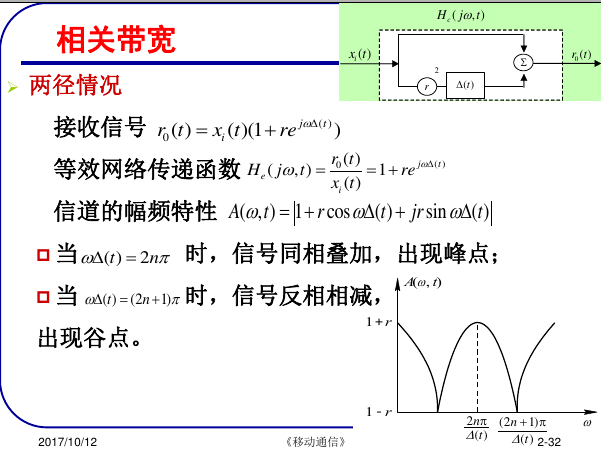
\includegraphics[width=0.7\linewidth]{figures/相关带宽退到.png}
			\caption{}
			\label{fig:}
		\end{figure}
		
}
	\item 空间选择性衰落,相关距离\footnote{在一定的空间距离,信道冲击响应能保证一定的相关度,这个空间距离就是相关距离(通长上就是接受天线防止的距离)}。
\end{enumerate}
\subsection{ 慢衰落特性和衰落储备
}
\subsubsection{满衰落}
定义:无线通信中,一般把由于距离引起的路径损耗和由于地形遮挡引起的阴影衰落统称为慢衰落,其衰落周期为秒级。
\begin{itemize}
	\item 天气引起的变化,更慢,小时或天级。
	\item 近似服从\textbf{对数正态分布}
\end{itemize}
\subsubsection{衰落储备}
 为了防止因衰落(包括快衰落和慢衰落)引
起的通信中断,在信道设计中,必须使信号的
电平留有足够的余量,以使中断率R小于规定
指标。这种电平余量称为衰落储备。\\
衰落储备大小决定于地形、地物、工作频率和要求的通信可靠指标(可通率T= 1-R)。\\
衰落储备可通过查表得到。

\section{陆地移动信道的传输损耗
}
\subsection{地形的分类
}
\begin{description}
	\item[中等起伏地形]地
	面起伏高度不超过20m。
	\item[不规则地形] 其余地形。
\end{description}
\textit{移动台天线的有效高度h 总是指天线在当地地面
	m上的高度。
}
\subsection{地物(地区)分类}
\begin{itemize}
	\item 市区
	\item 郊区
	\item 开阔地
\end{itemize}
\subsection{中等起伏地形上传播损耗的中值
}
奥村模型:适用范围:频率150MHZ ~1500MHZ,基
地站天线高度为30~200米,移动台天线高度为1~10
米,传播距离为1~20千米的场强预测。\\

基准中值:在计算各种地形、地物上的传播损耗
时,均以\textbf{中等起伏地}上的\textbf{市区},在\textbf{标准天
线高度,基站天线200m,移动台天线3m}下的损耗中值或场强中值作为基准,
称作基准中值或基本中值。其余情形将在
此基准上作修正。修正因子为实际场强中
值与基准场强中值之差。

\subsubsection{中等起伏地形损耗中值计算}
\begin{itemize}
	\item 自由空间损耗。+
	\item 传播损耗基准中值$A_m$(相对于自由空间的中值损耗),f,d越大$A_m$越大。+
	\item 基站天线高度增益因子 $ H_b $。天线越高,其值越大(天线越高,损耗越小)。-
	\item 移动台天线高度增益因子$ H_m $。天线越高,其值越大(天线越高,损耗越小)。-
	\item 街道走向修正因子 $ k_a $。纵向(与传播方向平行),大于0,横向(垂直),小于0。-
\end{itemize}
\begin{equation}\label{key}
L_t = L_{fs} + A_m - H_b - H_ -k_a
\end{equation}

\subsubsection{郊区和开阔地损耗的中值
}
\begin{equation}\label{key}
L_{\text{郊区}} = L_{\text{市区}} - K
\end{equation}
K为地形修正因子。\\
中等起伏地市区中接收信号的功率中值$ P_p $
\begin{equation}\label{key}
 P_p = P_0 - A_m + H_b + H_m
\end{equation}
$ P_0 $发送功率,其余地形技术算,即加上相应的地形修正因子。
\begin{equation}\label{key}
 P_p = P_0 - A_m + H_b + H_m+K_T
\end{equation}

\section{传播模型}
\begin{figure}[H]
	\centering
	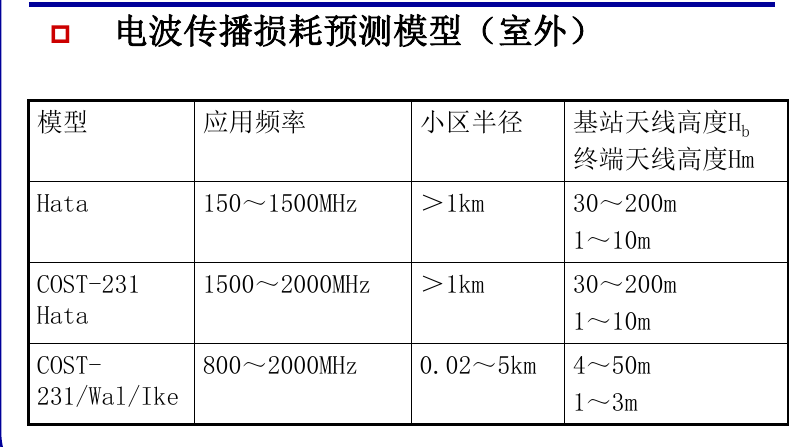
\includegraphics[width=0.7\linewidth]{figures/传播模型}
	\caption{}
	\label{fig:}
\end{figure}
